
\chapter{Motion Estimation}
\label{chapter:motion_estimation}

%\reviewcomment{To be written. Outline might evolve.}

\section{Introduction}

An important task in both human and computer vision is to model how images (and the underlying scene) change over time. Our visual input is constantly moving, even when the world is static. Motion tells us how objects move in the world, and how we move relative to the scene. It is an important grouping cue that lets us discover new objects. It also tells us about the three-dimensional (3D) structure of the scene.

Look around you and write down how many things are moving and what are they doing. Take note of the things that are moving because you interact with them (such as this book or your computer) and the things that move independently of you.

The first observation you might make is that not much is happening. Nothing really moves. Most of the world is remarkably static, and when something moves it attracts our attention. However, motion perception becomes extremely powerful as soon as the world starts to move. Our visual system can form a detailed representation of moving objects with complex shapes. Even in front of a static image, we form a representation of the dynamics of an object, as shown in the photograph in \fig{\ref{fig:050822_172806__MG_5366}}.

\begin{figure}[t]
    \centerline{
        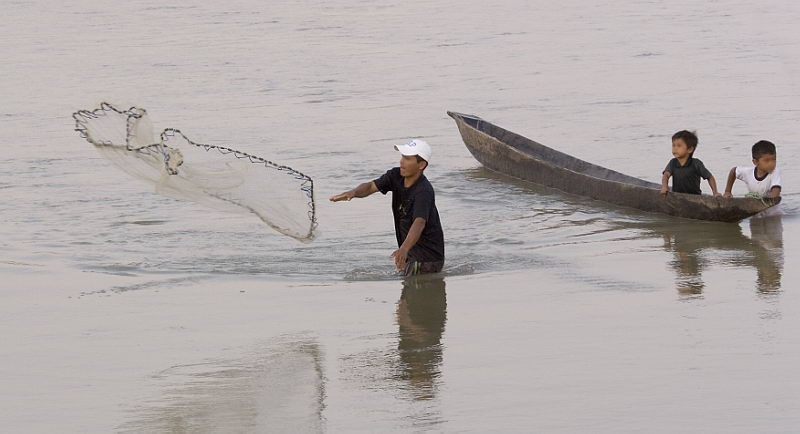
\includegraphics[width=.7\linewidth]{figures/optical_flow/050822_172806__MG_5366.jpg}
    }
    \caption{Even from a static picture we form a rich representation of the dynamics of the scene. {\em Source}: Photograph by Fredo Durand.}
    \label{fig:050822_172806__MG_5366}
\end{figure}

Looking at the power of that static image to convey motion, one wonders if seeing movies is really necessary. From the notes you took about what moves around you, probably you deduced that the world is, most of the time, static.

And yet, biological systems need motion signals to learn. Hubel and Wiesel \cite{Wiesel1981} observed that a paralyzed kitten was not capable of developing its visual system properly. The human eye is constantly moving with saccades and microsaccades. Even when the world is static, the eye is a moving camera that explores the world.

%\section{Definitions}

%longuet-higgins and Prazdny, 1980

%Scene flow

%Optical flow

%what is motion?

%what happens if the light moves. 

%how to describe the flow of smoke or water? rigid, deformable motion.

%\section{The perception of motion}


%Motion is also an important grouping cue. Scene points that move in the same way are likely to belong to the same object.  
Motion tells us about the temporal evolution of a 3D scene, and is important for predicting events, perceiving physics, and recognizing actions.
Motion allows us to segment objects from the static background, understand events, and predict what will happen next.  Motion is also an important grouping cue that our visual system uses to understand what parts of the image are connected. Similarly moving scene points are likely to belong to the same object. For example, the movement of a shadow accompanying an object, or various parts of a scene moving in unison—even when the connecting mechanism is concealed—strongly suggests that they are physically linked and form a single entity.

%%% gpt4 suggested the sentence above, instead of this, which I wanted improved:  For instance, the motion of a shadow that follows an object, or different parts of the scene that move coherently, even when the mechanism that connects them might be hidden from us, are potent indicators that they are physically connected and form a single entity. 




Motion estimation between two frames in a sequence is closely related to disparity estimation in stereo images. A key difference is that stereo images incorporate additional constraints, as only the camera moves—imagine a stereo pair as a sequence with a moving camera while everything else remains static. The displacements between stereo images respect the epipolar constraint, which allows the estimated motions to be more robust. In contrast, optical flow estimation doesn't assume a static world.

\marginnote{Disparity from stereo and optical flow estimations are closely related. Stereo benefits from the epipolar constraint to make estimation easier. For a rectified stereo pair the vertical component of motion between the stereo frames is zero.}[-1.5in]

Another distinction is that optical flow generally presumes small displacements between consecutive frames due to the short time gap between them. In stereo images, feature displacements tend to be larger. Despite these differences, the remaining steps are similar, and the same architectures can address both tasks.


\section{Motion Perception in the Human Visual System}


The eye is constantly moving, fixating different scene locations every 300 ms. Therefore, the nature of the input signal to the brain is a sequence of ever-changing visual information. It is not a surprise then that motion perception is a key component of visual perception.


\marginnote{Only when the eye tracks a moving object can it move continuously. Otherwise, the eye jumps from one location to another in saccades. Try moving your eyes smoothly and you will notice that you cannot. However, if you look at your finger you will see that you can follow its motion smoothly. }

What do we know about the human perception of motion?  Much is known and many advances from cognitive psychology have impacted imaging technology. One example is movies. The fact that we learned to create the illusion of continuous motion by displaying a sequence of static images (a phenomenon called {\bf apparent motion}) was a remarkable discovery. \index{Apparent motion}

There are a number of visual illusions associated with motion perception that are intriguing and offer a window into how motion perception is implemented in the brain. One famous illusion is the {\bf waterfall illusion}. When looking at a constant motion (such as a waterfall) our brain adapts to the motion in such a way that if, immediately after adaptation, we look at a static texture we will see it drifting in the opposite direction. The waterfall illusion was already known to the Greeks and was reported by Aristotle. Another remarkable and surprising visual illusion is that it is possible to create static images that produce the sensation of motion. One beautiful example is the {\bf Rotating Snakes} visual illusion created by cognitive psychologist Akiyoshi Kitaoka. \Fig{\ref{fig:motion_illusion}} shows an example a motion-inducing visual illusion, using very simple elements to produce the illusion. The effect becomes more intense as we move our eyes to explore different parts of the bicycle.  \index{Motion-inducing visual illusion}



\begin{figure}[t]
    \centerline{
        
\includegraphics[width=1\linewidth]{figures/optical_flow/moving_bike.eps}
    }
    \caption{Motion-induced visual illusion, after \cite{Murakami2010}. The illusion becomes stronger
        %when looking at the image with the eye periphery instead of looking directly to it. 
        when viewed peripherally rather than looking directly at the image. Changing the contrast of this image can change the direction of perceived motion.}
    \label{fig:motion_illusion}
\end{figure}
% https://commons.wikimedia.org/wiki/File:Anomalous_motion_illusion1.png

The opposite visual illusion can also be achieved: perceiving no motion when there is movement. By creating sequences with isoluminant and textureless patterns \cite{Sperling2017}, an observer can perceive them as perfectly still, even though they are moving. This illusion requires precise calibration and only works for the specific observer the system is tuned for; other observers will still see motion. The illusion can be thought of as an adversarial attack on a single observer's motion estimation system.

% I asked gpt4 to improve the paragraph below:(billf)
% What are the mechanisms used by the brain to translate the projected sequence of images on the retina onto actual motion on the 3D scene? Neuroscientists and psychologists have studied this problem for a long time. 
% Most visual neurons in area V1 of the visual cortex respond to moving stimuli and are selective to specific directions of motion. The motion selective neuron responds very strongly when an edge passes by its receptive field moving in a particular orientation and responds less as the direction of motion deviates from the preferred orientation. Many of this motion selective cells project to other specialized areas. There are two known areas in the cortex that seem to be heavily involved in the processing of motion: area MT and area MST. How exactly these areas work and what their role are is not completely understood yet. This organization seems to indicate that motion is processed by specialized visual pathways suggesting a modular architecture for the visual system. 

% I was happy with the result,  which I checked carefully:
What mechanisms does the brain use to translate the sequence of images projected on the retina into actual motion in the 3D scene? This question has long been studied by neuroscientists and psychologists.

In area V1 of the visual cortex, most visual neurons respond to moving stimuli and exhibit selectivity to specific motion directions. A motion-selective neuron responds strongly when an edge moves across its receptive field in a particular orientation, and its response diminishes as the motion deviates from the preferred direction. These motion-selective cells project to other specialized areas, with the middle temporal area (area MT) and the medial superior temporal area (area MST) playing significant roles in motion processing. The exact functions and roles of these areas are not yet fully understood. This organization suggests that motion is processed by specialized visual pathways, indicating a modular architecture for the visual system.

One of the early computational models of motion perception was proposed by Hassenstein and Reichardt \cite{hassenstein1956} when studying the motion detectors in the fly's visual system. Another computational model of human motion perception is the energy model proposed by Adelson and Bergen \cite{Adelson85} and briefly discussed in \chap{\ref{chapter:filter_banks}}. In this chapter we will focus on motion estimation algorithms developed by the computer vision community without trying to follow biologically plausible mechanisms.


\section{Matching-Based Motion Estimation}
\label{sec:matching_based_motion}
Let's get our hands dirty quickly by trying to estimate how pixels move in a video. Let's consider two frames of a video sequence that contains a few moving objects, as shown in \fig{\ref{fig:two_frames_from_palma_street}}.

\begin{figure}
    \centerline{
        \sublabel{Frame 1}{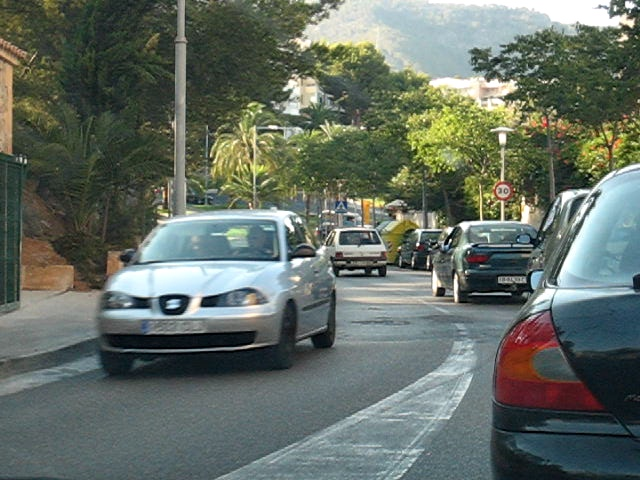
\includegraphics[width=0.48\linewidth]{figures/optical_flow/frame1.jpg}}
        \sublabel{Frame 2}{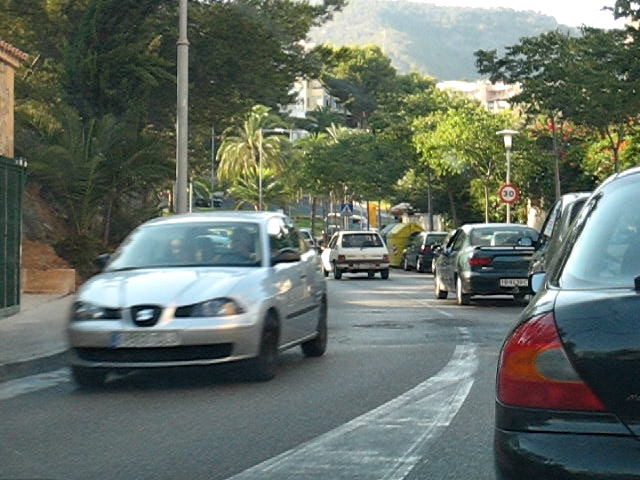
\includegraphics[width=0.48\linewidth]{figures/optical_flow/frame2.jpg}}
        %
        %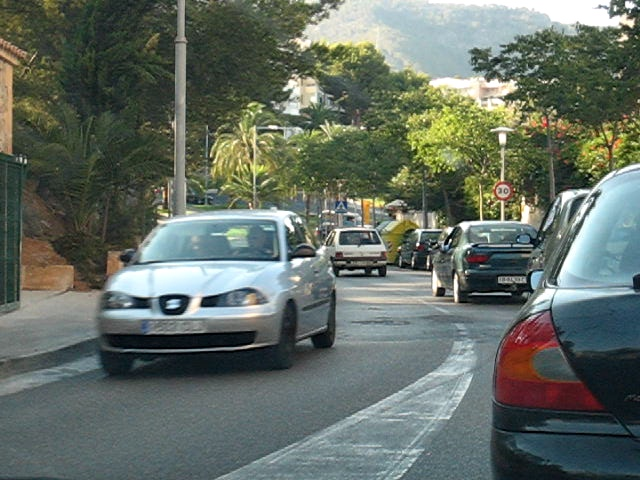
\includegraphics[width=0.495\linewidth]{figures/optical_flow/frame1.jpg}
        %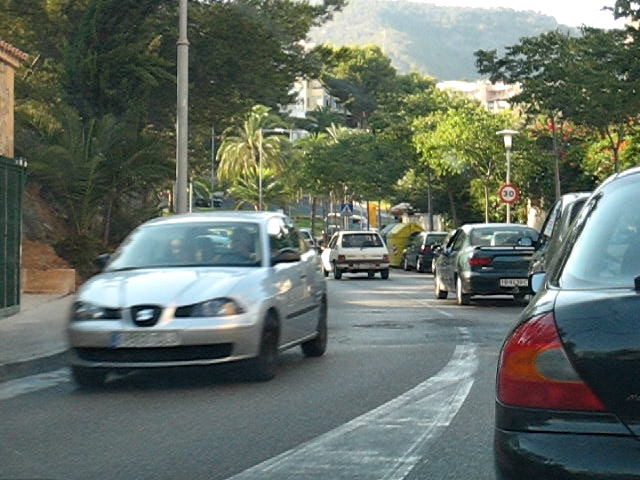
\includegraphics[width=0.495\linewidth]{figures/optical_flow/frame2.jpg}
    }
    \caption{Two frames of a video sequence captured from a moving car driving along a busy street in Palma de Mallorca (Spain).}
    \label{fig:two_frames_from_palma_street}
\end{figure}

These two frames belong to a sequence captured from a moving car driving along a busy street. In this sequence there are cars moving on both sides of the road, some moving away from the camera and others moving toward it.  How can we compute the motion between the two frames? One way of representing the motion is by computing the displacement for each pixel between the two frames.

Under this formulation, the task of motion estimation consists of finding, for each pixel in frame 1, the location of the corresponding pixel in frame 2. Just as in the chapter on stereo matching, we need first to define how we will compare pixels to find {\bf correspondences}. \index{Image correspondence}

Using the color of each individual pixel will be insufficient as many pixels are likely to have very similar colors. Instead we will represent each pixel by a color patch of size $C=3\times(2s+1)\times(2s+1)$ centered on each pixel. That is, for pixel in location $(n,m)$ in image $\boldimg$, we will use the patch $\boldimg [n-s:n+s, m-s:m+s]$ to represent the local appearance in that location. Small values of $s$ will result is small patches that might be less distinctive ($s=0$ corresponds to use individual pixels), while large values of $s$ will result in large discriminative patches but  might fail if there is sufficient geometric distortion between the two frames due to motion. By representing each pixel with a patch, we are transforming the image into a feature map of size $3\times(2s+1)\times(2s+1)$. As in \chap{\ref{chapter:perceptual_organization}}, we could also use other patch embeddings such as DINO or SIFT descriptors. But since the image transformation between two consecutive frames is usually small, using red-green-blue (RGB) patches can work well. Another constraint we can use to simplify the matching is to assume that motion will be small between the two frames so that we only need to look for matches inside a small neighborhood of size $L \times L$ in the second frame around the original pixel location. To compute distances between two patches we will use the Euclidian distance between them. We will then compute the motion at each pixel in the first frame by searching for the patch with the smallest distance in the second frame. We can implement this with the following algorithm:

\index{Patch matching}
\begin{algorithm}[h]
    \SetAlgoVlined
    \DontPrintSemicolon
    %\marginnote{{\bf Algorithm \ref{alg:motion_matching_algorithm}}: Patch matching motion estimation between two frames. The algorithm starts by chopping the two frames into overlapping patches. Then, for every patch from the first frame, we compute the distance to all the nearby patches in frame 2. Finally, for each input patch we select the closest patch from frame 2 and we record the relative displacement between the two patches. The pseudocode can be rearranged to be more memory efficient.}
    \caption{{\bf Algorithm \ref{alg:motion_matching_algorithm}}: Patch matching motion estimation. The algorithm starts by chopping the two frames into overlapping patches. Then, for every patch from the first frame, we compute the distance to all the nearby patches in frame 2. Finally, for each input patch we select the closest patch from frame 2 and we record the relative displacement between the two patches. The pseudocode can be rearranged to be more memory efficient.}
    \fakealgorithmcaption{}
    \label{alg:motion_matching_algorithm}
    {\bf Input frames:} $\boldimg_1, \boldimg_2 \in \mathbb{R}^{N \times M \times 3}$,
    {\bf Output motion flow:} $\mathbf{u}, \mathbf{v} \in \mathbb{R}^{N \times M}$\;
    {\bf Parameters:} $L = \text{Maximum displacement}, s = \text{Patch size parameter}$\;
    \For{\upshape $i = 0, \dots, M-1$}
    {
    \For{\upshape $j = 0, \dots, N-1$}
    {
    $\mathbf{r}_1[i,j] = \boldimg_1 [i-s:i+s, j-s:j+s] \quad \triangleleft \text{Chop up frame 1 into patches}$\;
    $\mathbf{r}_2[i,j] = \boldimg_2 [i-s:i+s, j-s:j+s] \quad \triangleleft \text{Chop up frame 2 into patches}$\;
    }
    }
    \For{\upshape $i = L, \dots, M-L-1$}
    {
        \For{\upshape $j = L, \dots, N-L-1$}
        {
            \For{\upshape $di = -L, \dots, L$}
            {
                \For{\upshape $dj = -L, \dots, L$}
                {
                    $C[i,j][d_i,d_j] = \text{dist}(\mathbf{r}_2[i+di,j+dj], \mathbf{r}_1[i,j])
                        \quad \triangleleft \text{Compute matching cost}$\;
                }
            }
        }
    }
    \For{\upshape $i = L, \dots, M-L$}
    {
        \For{\upshape $j = L, \dots, N-L$}
        {
            $\mathbf{u}[i,j] = \argmin (\min (C[i,j], axis=1)) \quad \triangleleft \text{Estimate  displacement x}$\;
            $\mathbf{v}[i,j] = \argmin (\min (C[i,j], axis=0)) \quad \triangleleft \text{Estimate  displacement y}$\;
        }
    }
\end{algorithm}


Note that padding must be applied if we want to compute the output optical flow near the image boundaries. Algorithm \ref{alg:motion_matching_algorithm} could be written more compactly but we prefer this form for its clarity. The following images shows the matching result for one input location. In this example, $s=5$ (patch size of $11\times11$ pixels), and $L=16$ (search window of size $33\times33$ pixels).



In the example shown in \fig{\ref{fig:matching_cost_figure}}, the input patch is centered on the car logo. The matching cost displays the distance using a reversed grayscale map, with smaller values appearing as brighter spots. In this case, the search identifies a unique match. However, it is worth noting that the best matching patch, although correctly detecting the same logo, is not identical to the input patch. This discrepancy can be attributed to factors such as nondiscrete motion and the slight enlargement of the logo as the car approaches the camera.


\begin{figure}[h!]
    \includegraphics[width=1\linewidth]{figures/optical_flow/matching_cost_figure.eps}
    \caption{Two frames and best match for an input patch from frame 1 within frame 2. Search is done only within a small neighborhood.}
    \label{fig:matching_cost_figure}
\end{figure}

The patch size used to represent each pixel is the most important parameter in this algorithm. \Fig{\ref{fig:matching_optical_flow_patch_size_effect}} shows the effect of the choice of the parameter $s$ on the estimated optical flow.


\begin{figure}[h!]
    \centerline{
        \includegraphics[width=.8\linewidth]{figures/optical_flow/matching_optical_flow_patch_size_effect.eps}
    }
    \caption{Effect of the choice of the patch size parameter, $s$, on the estimated optical flow. When the patch size is just one pixel ($s=0$), the approach fails as there are many similar pixels that correspond to different parts of the scene. Only when the patches are large enough, the image matches correspond to the same scene elements. Large patch sizes are necessary. But too large patches lead to oversmoothing. }
    \label{fig:matching_optical_flow_patch_size_effect}
\end{figure}

When using single pixels to represent each location, the matching fails in detecting true correspondences and the estimated motion field is very noisy. Just making the patches $5 \times 5$ pixels is already capable of detecting many correct matches and the motion field seems to mostly capture the true motion between the two frames. Further increasing the patch size eliminates some of the errors. However, using very big patches also introduces new problems. In this example we can see how the motion of the gray car extends over the road. This is due to patches overlapping with the car on top, and as the road is mostly uniform, the motion of the car propagates to all the nearby pixels. One of the challenges in this algorithm is that the ideal value of $s$ will depend on the sequence.


This approach has many shortcomings. To start, we assumed that motion is discrete (it can only take on integer values). Therefore, the current approach does not compute displacements of pixels to subpixel accuracy that might be important if we need precision or if motions are very small. We could improve the approach by interpolating the cost function or by computing subpixel displacements using bilinear or bicubic interpolation, but it would become more computationally expensive. In addition, the patch matching method gives poor results near motion discontinuities such as object edges.

%The representation also treats motion as a 2D vector, when it fact is the result of motion happening in a 3D world. 

One advantage of this algorithm is that motion is computed in a way that is independent of the objects present in the scene. We did not make any assumption about what objects are moving or how. We did not introduce any grouping cues (as in \chap{\ref{chapter:perceptual_organization}}) to presegment the image into candidate objects. Therefore, we could use the computed motion as new cue for grouping.



\section{Does the Human Visual System Use Matching to Estimate Motion?}
%\reviewcomment{Figures need reformatting.}

While researchers aren't sure of the precise computations involved in human motion processing, some experiments can distinguish between classes of algorithms that the visual system may use.  The previous method is an example of {\bf pattern matching methods} \cite{Adelson85}, which are often based on image correlations. A second class of motion algorithms are based on {\bf spatiotemporal filtering} \cite{Adelson85} and their principles were briefly described in \chap{\ref{chapter:filter_banks}}. Spatiotemporal filtering uses the responses of velocity-tuned filters to estimate the motion.

%are based on {\em spatio-temporal filtering} \cite{Adelson85}.  A second class of motion algorithms includes correlation-based methods, and can be called {\em pattern matching methods} \cite{Adelson85}.  In such methods, the motion offset of a spatial pattern from some starting position is computed by finding the position of highest correlation with the spatial pattern.

Adelson and Bergen proposed a beautiful motion illusion that distinguishes between two classes of motion algorithms that might be used by the visual system (\fig{\ref{fig:motionIllusion1}}).  The illusion involves temporal filtering, motion processing, and aliasing and thus provides a good review of the material in this chapter and also chapters \ref{chapter:sampling} and \ref{chapter:temporal_filters}.



\begin{figure}[t]
    \centerline{
        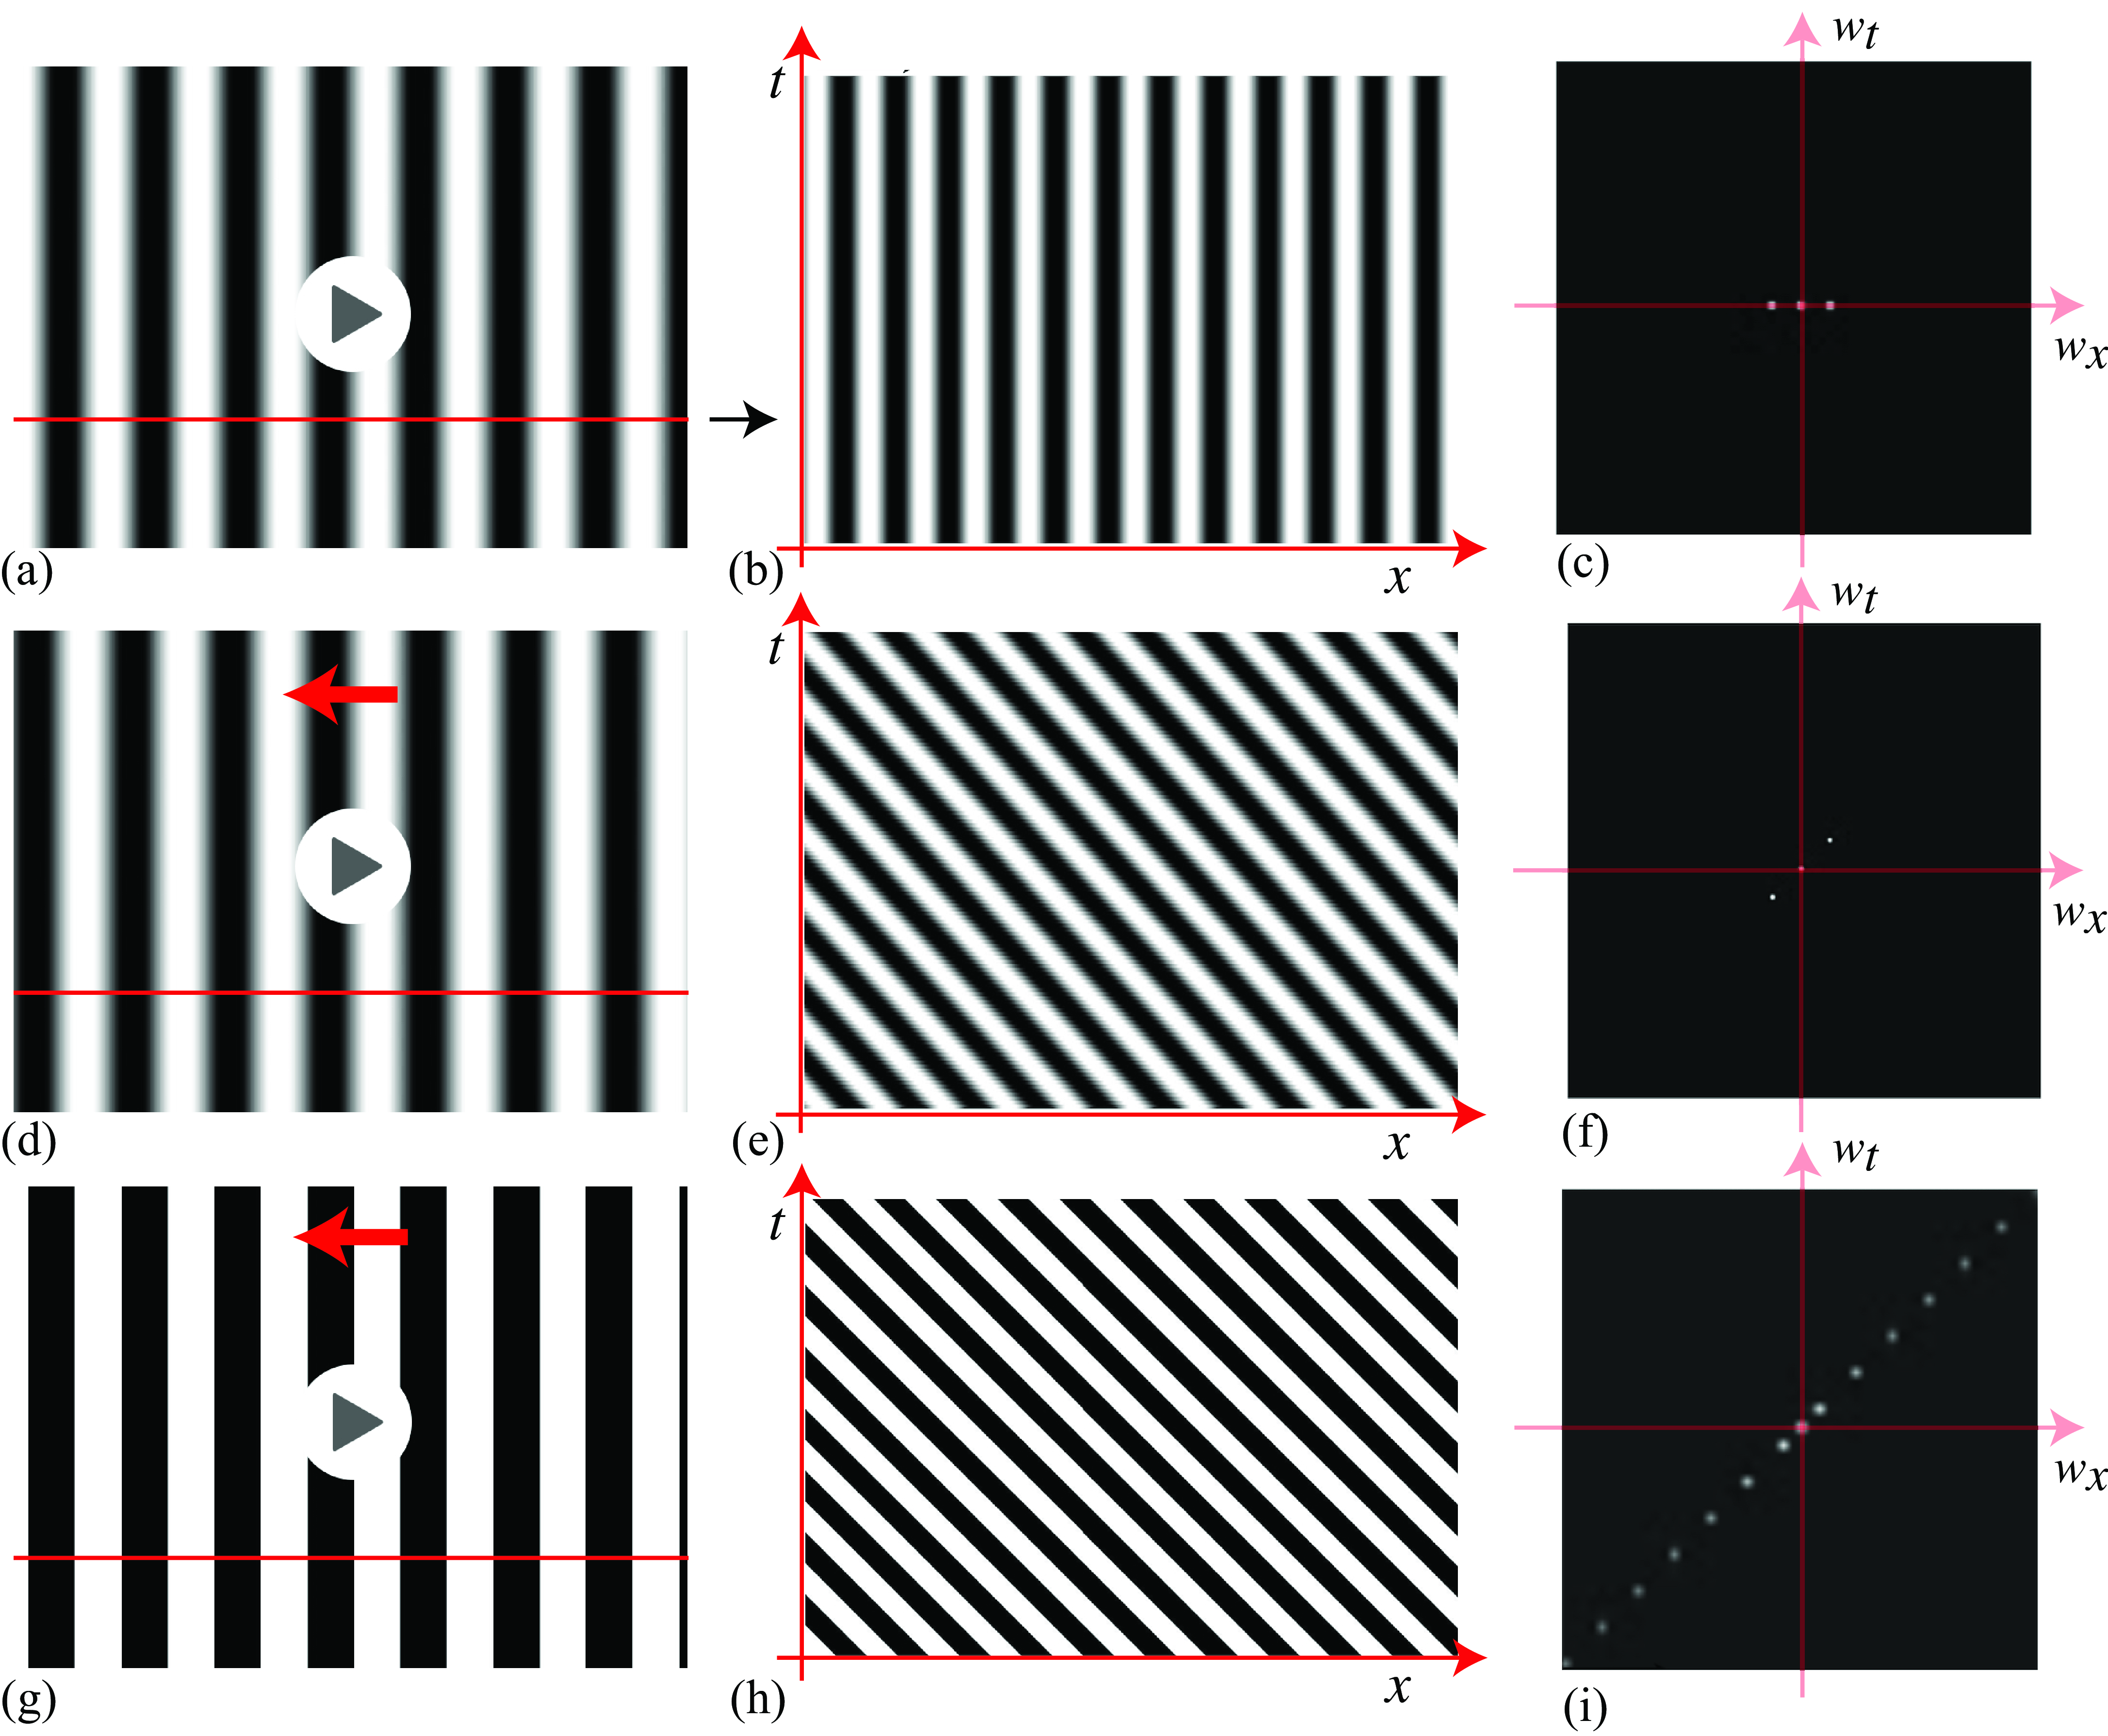
\includegraphics[width=1\linewidth]{figures/optical_flow/ted_demo_motion_1.eps}
    }
    \caption{Space-time signals, building toward the fluted square-wave motion illusion. The first row shows a stationary sine wave. (a) Movie of a motionless sine wave. (b) Space-time plot shows only vertical structure. (c) Spatiotemporal Fourier transform shows all energy on the zero temporal frequency axis because nothing is moving. (d) The second row shows a moving sine wave. (e) In the space-time plot, speed corresponds to
        local orientation. (f) The Fourier transform energy is sheared according to
        the sine wave’s speed. (g–i) The third row shows a moving square wave. The additional harmonics required to form a square wave are visible in (i) the spatiotemporal Fourier transform.
        %First row: stationary sine wave, (a) Movie of a motionless sine wave. (b) The space-time plot shows only vertical structure. (c) spatio-temporal Fourier transform has all energy on the zero temporal frequency axis, since nothing is moving. Second row:  (d) moving sine wave. (e) In the space-time plot, speed corresponds to local orientation. (f) The Fourier transform energy is sheared according to the sine wave's speed.   Third row:  Moving square wave.  The additional harmonics required to form a square wave are visible in the spatio-temporal Fourier transform, (i).
    }
    \label{fig:motionIllusion1}
\end{figure}


%The illusion is presented in the video in \fig{\ref{fig:blends}}. 
The signals, and magnitudes of their space-time Fourier transforms, are developed in figures~\ref{fig:motionIllusion1} and \ref{fig:motionIllusion2}, building-up from simpler signals.  The three rows of \fig{\ref{fig:motionIllusion1}} show a stationary sinusoid, a moving sinusoid, and a moving square wave.  The spatiotemporal Fourier transform of the stationary sinusoid, $f(x,y,t) = \cos(\pi \omega x)$, is $(\delta(w_x + \omega) + \delta(w_x - \omega)) \delta(w_y) \delta(w_t) $.  We have added a constant bias to the sinusoid to avoid negative intensity values, leading to an impulse at the center of the Fourier transform, as shown in \fig{\ref{fig:motionIllusion1}}{c}.  The resulting three colinear impulses are along the temporal frequency, $w_t = 0$ line.  A space-time plot of the signal (\fig{\ref{fig:motionIllusion1}}[b]) shows only vertical structures, indicating no motion.

A moving sinusoid has a similar Fourier transform magnitude (\fig{\ref{fig:motionIllusion1}}[f]) but with the spatiotemporal energies along a line perpendicular to the moving structures in the spatiotemporal signal (\fig{\ref{fig:motionIllusion1}}[e]).  A moving square wave is similar, but the extra harmonics needed to construct the square wave visible in the Fourier transform (\fig{\ref{fig:motionIllusion1}}[i]).

Continuing the development of the illusion, \fig{\ref{fig:motionIllusion2}}{c} shows the Fourier transform and space-time plot of a square wave moving in 1/4 period jumps each time increment.  This signal can be formed from \fig{\ref{fig:motionIllusion1}}{h} by applying a periodic sample-and-hold function, resulting in the spectrum of  \fig{\ref{fig:motionIllusion1}}{i} replicated over temporal frequencies, and multiplied by a sinc function over temporal frequency.  The resulting Fourier transform magnitude is shown in \fig{\ref{fig:motionIllusion2}}{c}.


\begin{figure}[t]
    %\centerline{
    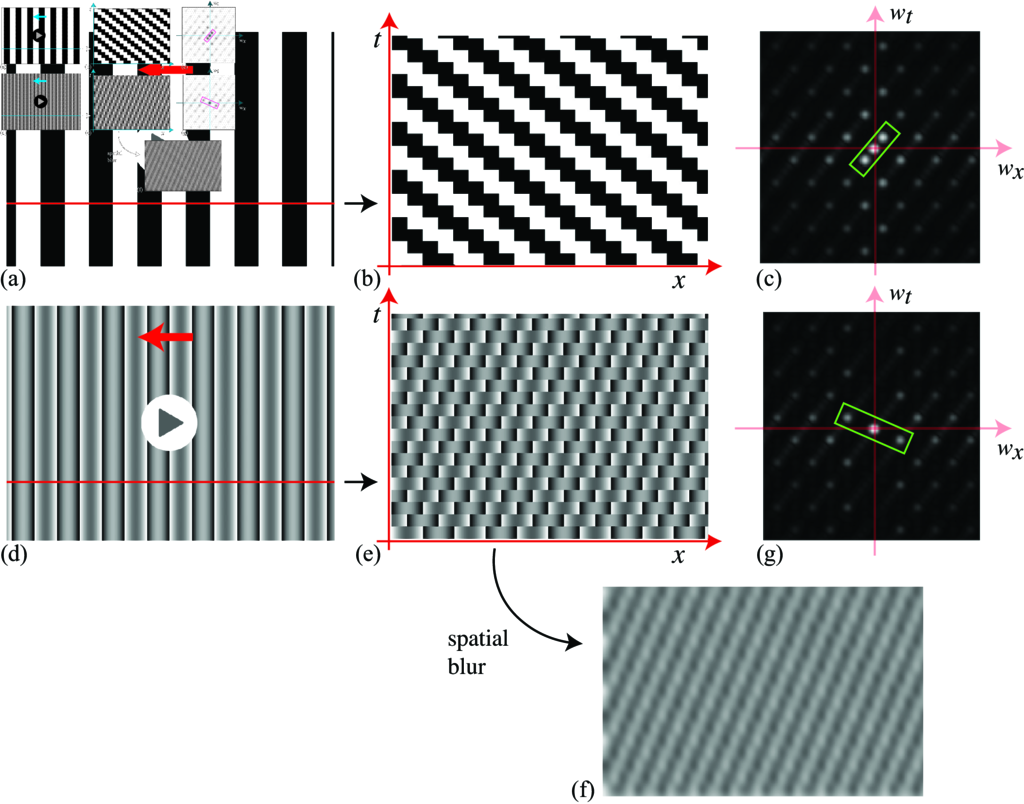
\includegraphics[width=1\linewidth]{figures/optical_flow/ted_demo_motion_2.eps}
    %} 
    \caption{Derivation of the fluted square-wave motion illusion, continued from \fig{\ref{fig:motionIllusion1}}. Top row shows that the square wave moves in 1/4 wavelength jumps, instead of continuously. This staggered motion generates the additional spatiotemporal frequencies shown in (c).  The lowest spatiotemporal frequency (green rectangle) still indicates motion to the left.  Second row shows that if we remove the lowest spatial frequency sine wave of the square wave, creating a {\em fluted square wave}, then the lowest spatio-emporal frequency now moves in the other direction.  This is also visible from (e) the space time plot and especially in (f) the spatiotemporally low-pass filtered version.}
    \label{fig:motionIllusion2}
\end{figure}

Because orientation in space-time tells motion direction (\sect{\ref{sect:modelingSequences}}) the space-time plot of \fig{\ref{fig:motionIllusion2}}{b} shows that the motion should be perceived to the left.  This will be consistent with the behavior of velocity tuned filters (\sect{\ref{sect:velocityTunedFilters}}) responding to the lowest spatiotemporal frequency impulses shown in
\fig{\ref{fig:motionIllusion2}}{c}. However, if we remove the lowest spatial frequency sinusoid from the signal, the result is shown in
\fig{\ref{fig:motionIllusion2}}{e}, with spatiotemporal Fourier transform shown in \fig{\ref{fig:motionIllusion2}}{g}.  Now the lowest spatiotemporal frequency cosine wave is oriented in the other direction.  This opposite slope is also visible in the spatial domain, in the space-time plot of \fig{\ref{fig:motionIllusion2}}{e}, and especially if we apply a low-pass filter, resulting in \fig{\ref{fig:motionIllusion2}}{f}.

The signal of the second row of \fig{\ref{fig:motionIllusion2}} poses a conundrum.  It can be argued that the signal moves to the left, just as does the signal of row 1 of \fig{\ref{fig:motionIllusion2}}.  The pattern match, that is, the minimum correlation signal indeed moves to the left.  But the vision system examining the orientation of the lowest spatiotemporal frequency components of the signal in \fig{\ref{fig:motionIllusion2}}{g}, or looking at the dominant orientations in the space-time plots of figures~\ref{fig:motionIllusion2}(e and g), would find a signal moving to the right!  Videos showing each signal are available on the book's web page.  These illusions give support to the spatiotemporal energy models for human motion processing.

%How does the signal appear to move to you?  We invite you to play the videos of \fig{\ref{fig:motionIllusion2}}{c} and (g) (set your player to loop the videos) to assess which way each of the signals of  \fig{\ref{fig:motionIllusion2}} moves.   \fig{\ref{fig:blends}} show slow and fast motion versions of a blended signal, where the top half contains the lowest sinusoidal spatial frequency component of the square wave and the bottom half does not.  By moving your eye vertically, you can convince yourself that the entire pattern is moving rigidly to the left, yet it also appears that the top half is moving to the left and the bottom half is moving to the right.  This demonstration gives evidence for spatio-temporal filter-based motion processing within the human visual system, since such filtering would predict leftward motion for the top halves of the videos in Fig.~\ref{fig:blends}, and rightward motion for the bottom halves of those videos.





%\begin{figure}[t]
%\centerline{
%\sublabelnp{(a) 
%\href{https://groups.csail.mit.edu/vision/cvbook/videos/blendedSlowLoop.mov}{
%motion illusion, slow (click for video)
%}
%}
%{
%\href{https://groups.csail.mit.edu/vision/cvbook/videos/blendedSlowLoop.mov}{
%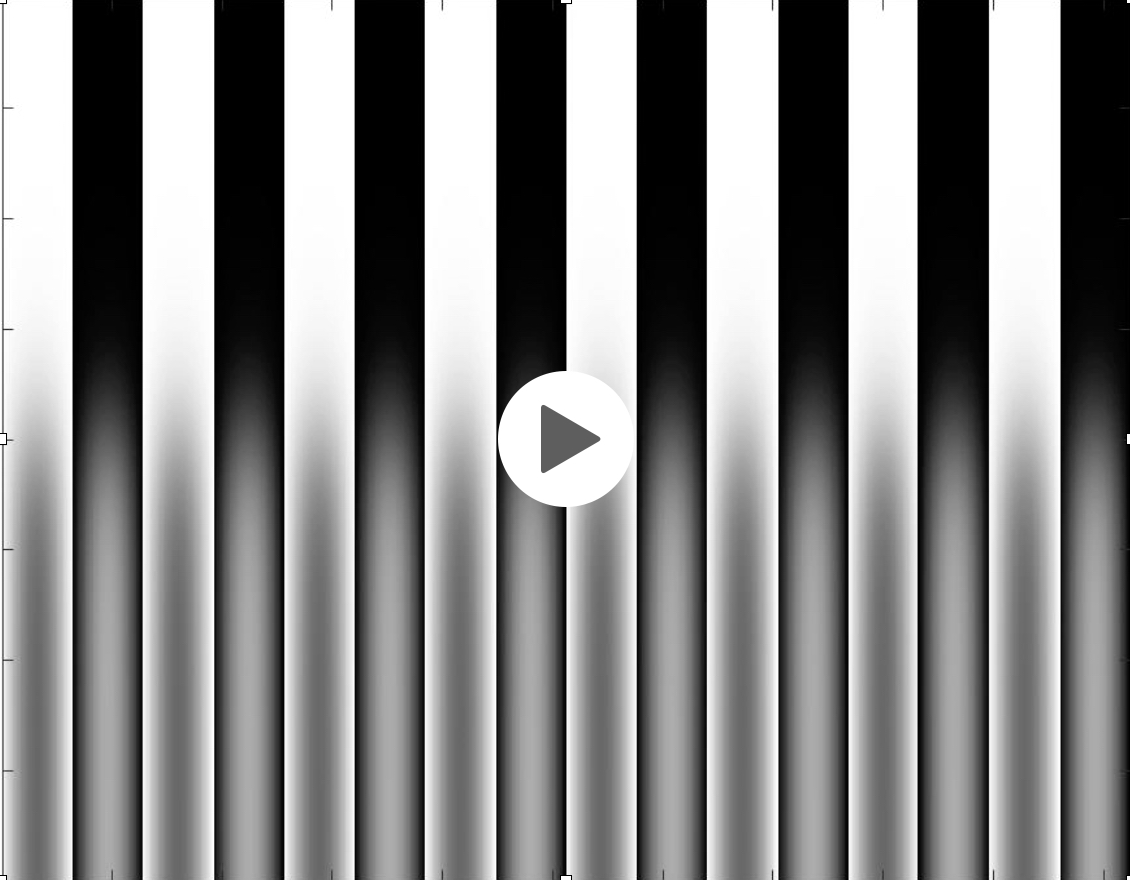
\includegraphics[width=0.5\linewidth]{figures/temporal_filters/blendFrame.jpg}}
%}
%\sublabelnp{(b) 
%\href{https://groups.csail.mit.edu/vision/cvbook/videos/fastBlendLoop.mov}}
%{
%\href{https://groups.csail.mit.edu/vision/cvbook/videos/fastBlendLoop.mov}{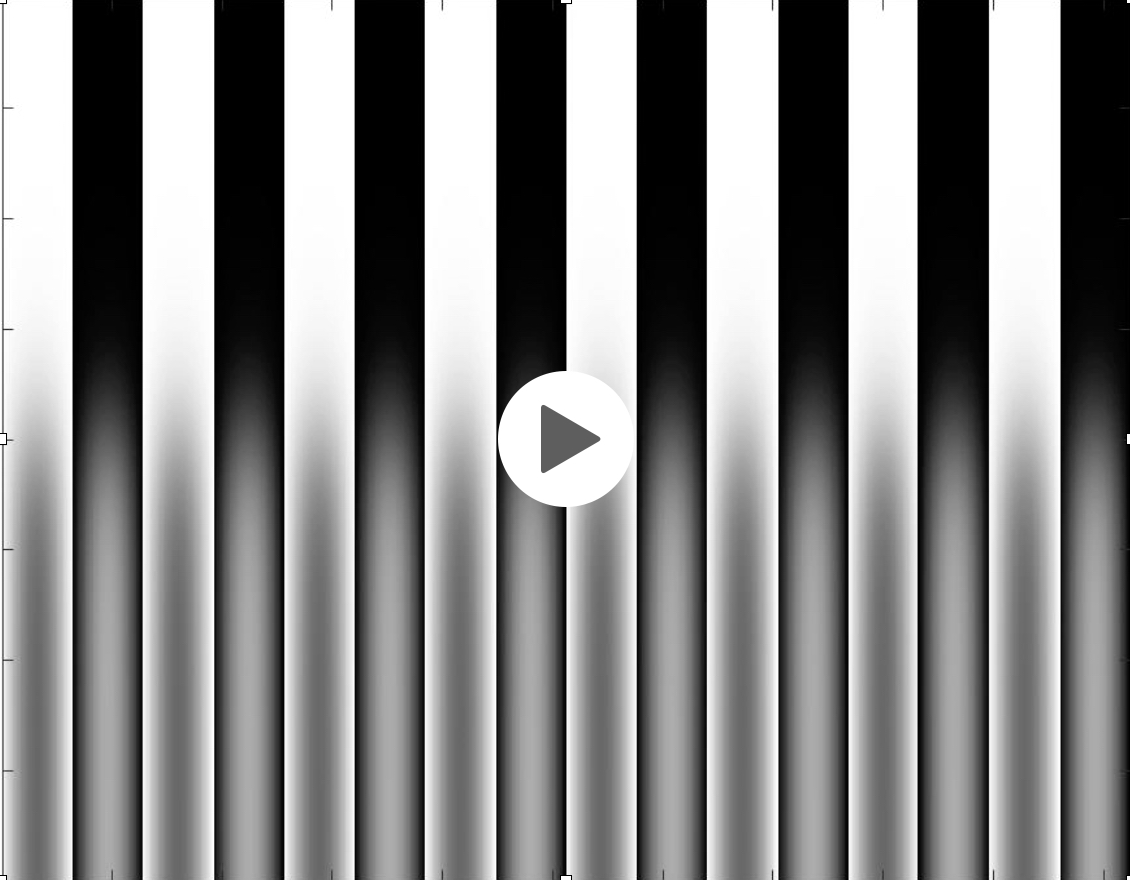
\includegraphics[width=0.5\linewidth]{figures/temporal_filters/blendFrame.jpg}}}
%}
%\caption{"Impossible combination" of ordinary and  fluted square-waves (view on looping display).  While one can verify, by tracing a finger or scanning your eyes, that the entire structure is moving rigidly to the left, the bottom half appears to be moving to the right.  At a fast speed, (b), the effect is accentuated.}
%\label{fig:blends}
%\end{figure}



\section{Concluding Remarks}

In this section we have introduced a conceptually simple approach to compute the motion in sequences. But are the estimated patch displacements meaningful? Do they correspond in any way to the motion in the 3D world?

We have computed motion between two frames before really understanding the motion formation process (i.e., how a camera looking at a moving 3D scene produces two-dimensional [2D] sequences). How should the correct motion look? And what do we want to do with it?
So, before we move into more sophisticated motion estimation algorithms, let's revisit the image formation process and examine how motion on the image plane emerges from the perspective projection of a dynamic 3D scene into a moving camera.
